\documentclass{ucb}
\usepackage{cleveref}

\begin{document}
\ucbcourse{\textbf{ASEN 6037} Turbulent Flows}
\ucbtitle{Literature Review: \textit{A Hybrid {{RANS}}-{{LES}} Approach with Delayed-{{DES}} and Wall-Modelled {{LES}} Capabilities}}
\ucbauthors{James Wright \\}
\ucblocation{Boulder, Colorado}
\ucbcover{}

\section{Introduction}
This literature review will cover the content and background of \citetitle{shurHybridRANSLESApproach2008}\cite{shurHybridRANSLESApproach2008}. 

\section{Summary of Prior Work}
This paper introduces a new hybrid RANS-LES turbulence model, later known as the improved delayed detached eddy simulations (IDDES). Before reviewing the paper, let's review the history of hybrid turbulence models in general.

IDDES can trace it's main roots back to the seminal detached eddy simulation (DES)~\cite{SpalartP.R.JouW-H.StreletsM.Allamaras1997} model, first proposed by \citeauthor{SpalartP.R.JouW-H.StreletsM.Allamaras1997}. The concept and motivation of hybrid models is fairly simple. LES is very expensive (particularly near the wall) for high Re flows, while RANS is significantly cheaper but not reliably accurate for many types of flow problems. Hybrid models combine the two to exploit their strengths and cover up their weakness. In general, RANS is responsible for flow regions that are very expensive for LES (namely near the wall) and LES is responsible for regions where RANS is not adequate. This is visually shown in \cref{fig:HRLMS}, where the shaded regions represent the parts of the turbulent spectrum that are modeled.

\begin{figure}[h]
    \centering
    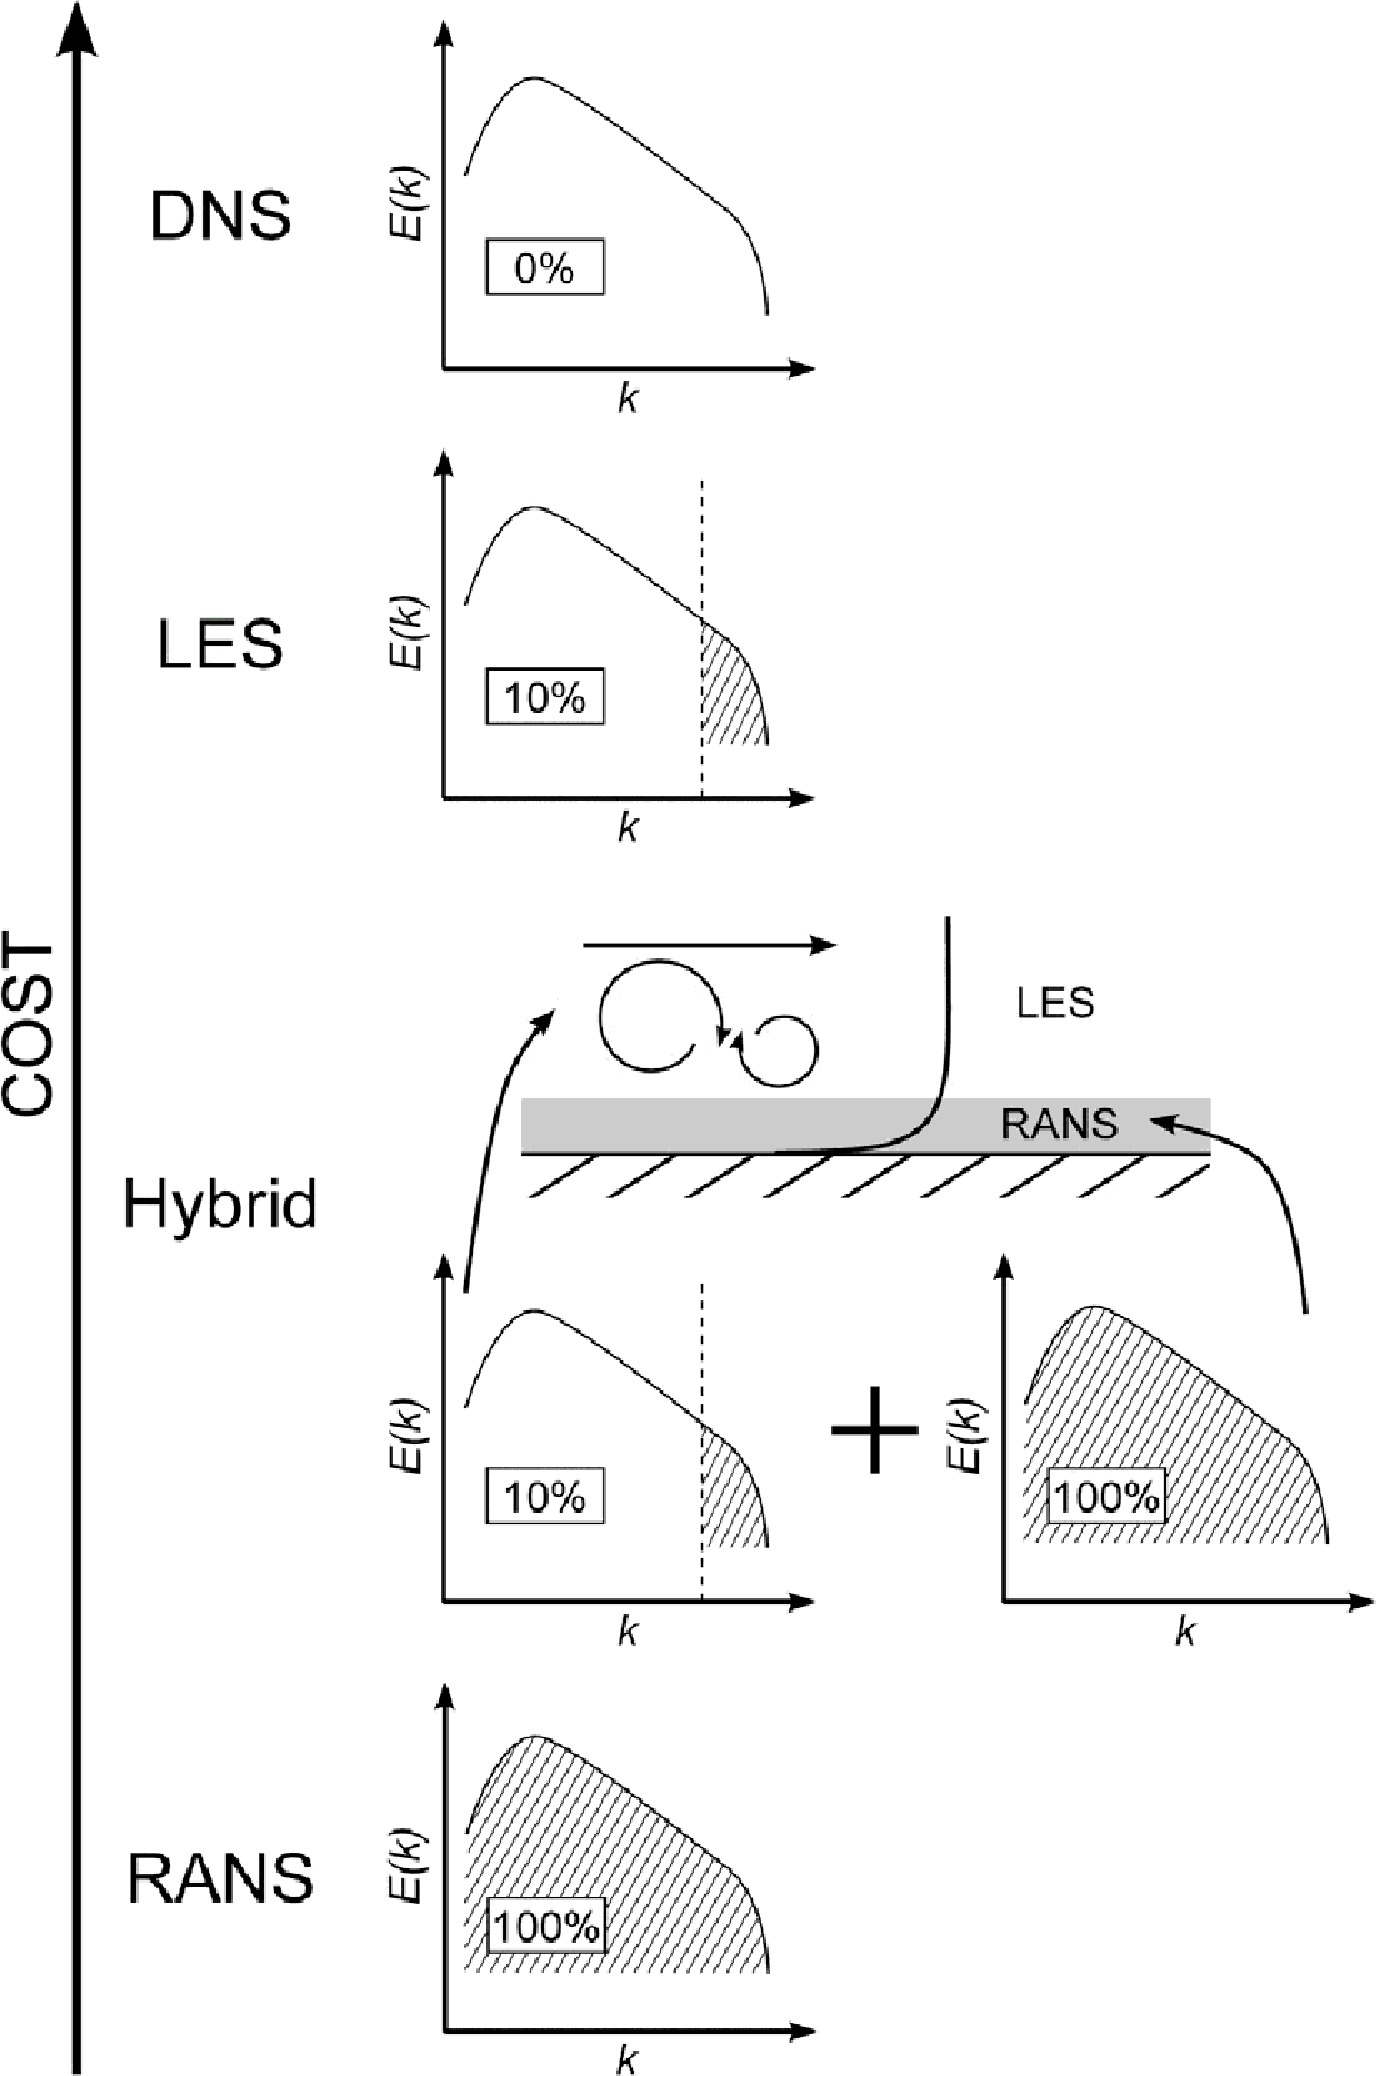
\includegraphics[]{img/TurbulenceModelsResolution_Tucker2015.jpg}
    \caption{Turbulence model hierarchy. Reproduced from~\cite{Tucker2015} under the Creative Commons Attribution License (\url{https://creativecommons.org/licenses/by/4.0/}).}
    \label{fig:HRLMS}
\end{figure}

% While there are some conceptual issues with the original DES formulation, %! reference to desire for WMLES instead of RANS near wall
The transition between the two models is one of the primary achilles's heel of DES-like methods. This is true both in determining where transition should occur and in transforming the modeled stress in the RANS region into resolved turbulence structures required by LES. The transition point was the primary reason for the first (of many) modifications to the original DES model. The DES model based the transition point on the grid size. This lead to issues (Modeled Stress Depletion and consequently Grid Induced Separation) when the model was used on different sized near-wall grids. This issue was addressed by \citeauthor{Menter2002} in \citedate{Menter2002} by introducing a shielding function to the DES formulation~\cite{Menter2002}. The original transition mechanism in DES was suppressed inside a boundary layer, as determined by the shielding function. This idea was originally only implemented with the SST-based DES model, but was generalized into the delayed detached eddy simulation (DDES) by \citeauthor{Spalart2006} in \citedate{Spalart2006}~\cite{Spalart2006}.

One other undesirable consequence of the model transition is termed the log-layer mismatch, referring to the log-layer of the boundary layer. The the issue is that while both RANS and LES both accurately predict the logarithmic relationship between \(u^+\) and \(y^+\), they predict them at different magnitudes. This relationship has been shown to occur

\section{Work Summary}
This work introduces a new hybrid RANS-LES turbulence model, which was later dubbed improved delayed detached eddy simulation (IDDES). This model builds on previous work on hybrid turbulence models by introducing a new function that allows the model to enter a wall-modeled LES mode.

\ucbbib{}
    
\end{document}